\documentclass{article}
\usepackage[utf8]{inputenc}
\usepackage{graphicx}
\usepackage{amsmath}
\usepackage{amsfonts}
\usepackage{geometry}
\geometry{
a4paper,
total={170mm,257mm},
left=20mm,
top=20mm}
\usepackage{graphicx}

\renewcommand{\figurename}{Abbildung}


\title{ \textbf{Skyhook Projekt} \\ \textmd{Eine Infrastruktur zwischen Erde und Mars}}  % \\ \textmd{}

\author{
  Quentin Wach \\
  Fabian Heisinger \\
  Otto Markmann
  \date{2. August bis 10. Oktober 2019}
}

\begin{document}
\maketitle
\begin{abstract}
Traditionelle Raumfahrt ist teuer, gefährlich und unfassbar Ressourcen-intensiv. Ein einfacherer Weg  ins All zu kommen ist ein sogenannter Skyhook oder Spacetether,  ein ständig rotierendes Seil, das Raumschiffe wie ein Katapult aus dem Orbit ins All schießt. Wir simulieren eine Skyhook Infrastruktur im Sonnensystem.
\end{abstract}
\begin{center} 
	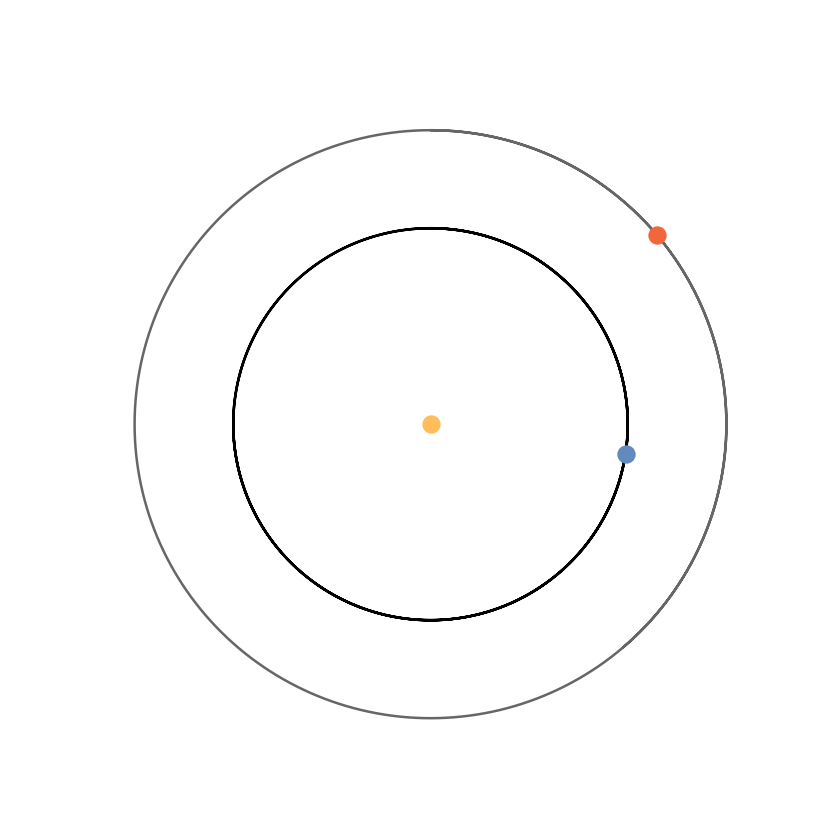
\includegraphics[width=200px]{../Abb/Abb_1.png}	
\end{center}
\section{Hintergrund}
Treibstof macht ca. 80$\%$ der Masse moderner Raketen aus []. Dessen Aufgabe besteht hauptsächlich darin das eigentliche Raumgefährt in einen Orbit zu bringen. Eine Infrastruktur zur Vereinfachung von Raumreisen setzt genau hier an und vermindert mit Senkung der zu erreichenden Flughöhe auch den Anteil des nötigen Treibstoffs. Eine Raumstation im Orbit, der Skyhook, mit einem tief über der Erdoberfläche hängendem Dock...

\section{Umsetzung}
\subsection{Sonnensystem}
Wir betrachten lediglich Erde und Mars im Umlauf um die Sonne in der x-y-Ebende. Es werden die Keplerregeln zunächst vernachlässigt und die Bahnen der Planeten als Kreise aufgefasst. Die Abstände zur Sonne werden dabei zeitlich gemittelt. Beide Planeten werden ebenfalls als Kreise mit diskreten Radien beschrieben. Ihre Umlaufzeiten variieren wie auch ihre Radien, Massen und Abstände zur Sonne. 

 
\subsection{Raumfahrtzeug}
Das Projektil wird von der Erde zu gegebenen Zeitpunkt abgefeuert
\subsection{Interplanetarischer Ballistischer Flug}
Um von einem Planeten zum nächsten zu gelangen muss die Rakete zunächst die Erde verlassen. Das Erreichen der dazu nötigen Fluchtgeschwindigkeit ist jedoch nur ein Teil des Problems zu dem außerdem das Gravitationsfeld der Sonne und die Bewegung der Erde um die Sonne betrachtet werden muss. Es wird diese höhere Rotationsgeschwindigkeit der Erde um die Sonne als die des Mars genutzt, um diesen - wenn nötig - einzuholen. Eine Beschleunigung des Geschosses in Bewegungsrichtung der Erde, also tangential zur Bahn, führt zu einer elliptischen Bahn mit zeitweise weiterer Ausdehnung der Bahn, so dass das Erreichen des Mars oder anderen höheren Orbits möglich wird. Umgekehrt führt eine Verlangsamung des Geschosses zu einer Reduktion der Orbithöhe. 

Da die Massen der Planeten im Vergleich zur Sonnenmasse äußerst gering sind, werden deren gravitativen Einflüsse zunächst ignoriert. Die Bahn des Geschosses wird numerisch genähert. Dabei wird davon ausgegangen, dass sich die Intervalle linear annähern lassen, also $\Delta v = \frac{\Delta s}{\Delta t}$. Mit jedem Zeitschritt (in Tagen) wird der Schritt durch die Gravitation $\Delta s_G$ und der Schritt durch die eigene Geschwindigkeit $\Delta s_v$ seperat ermittelt und dann summiert:

\begin{align*}
\Delta \vec{s_G} = -\frac{G \cdot M}{(x^2 +y^2)^{1,5}} \cdot \begin{pmatrix}x \\ y\end{pmatrix} \qquad \text{und} \qquad
\Delta \vec{s_v} = \vec{v} = \begin{pmatrix} \Delta x \\ \Delta y \end{pmatrix}
\end{align*}
Also
\begin{align*}
\Delta \vec{s} = \Delta \vec{s_G} + \Delta \vec{s_v}.
\end{align*}
Dabei ist $G = 6,67430(15) \cdot 10^{-11} \frac{\text{m}^3}{\text{kg} \cdot \text{s}^2}$ die Gravitationskonstante, und $M = (1,98892 \pm 0,00025) \cdot 10^{30} \text{kg}$ die Masse der Sonne. Das Zeitelement fällt hier weg, da es gleich Eins ist. Wir betrachten die zurückgelegte Strecken in $\frac{\text{km}}{\text{Tag}}$.
 
\section{Diskussion}



\end{document}
